\chapter{main\_LuaTeX.texの設定}
基本的に\TeX Wiki~\cite{luatex}や美文書作成入門~\cite{美文書作成入門},
main\_LuaTeX.texのコメントアウトを読めばわかるようにしているつもりである.
このテンプレートは2023年度高知工科大学 電子・光システム工学教室(以降,電子系と称する)の卒業論文・修士論文の要件を
満たすように作成したつもりだが、\textcolor{red}{今一度学位論文の要件を確認すること.}
作成者はこのテンプレートを用いることによる不利益に関しては保証しかねるのでご容赦を。。。
プリアンブルなどを調節したい場合は各自で行うこと.

このテンプレートは,ローカルではWindows10とWindows11のVisual Studio Codeで,
オンラインではOverleafとCloud LaTeXで動作実証済み($2023$年$12$月現在).
ただし,ローカルの場合は\TeX Live 2023で\LaTeX をインストールすることを前提としている.
\TeX Live以外にMac\TeX があるらしいが詳しいことは知らない.

\section{ここで使用する\LaTeX}
この \LaTeX はLua\TeX -jaを採用している.
Lua\TeX は従来のp\LaTeX とは異なりDVIファイルを経由せずに直接PDFを生成する.
また,Unicodeにも対応しており,たとえばSchr\"odinger (シュレーディンガー) を入力する際に
Schr\textbackslash "odingerとする必要はなく
そのままSchrödingerとしてもエラーを吐かずに出力してくれる(地味にありがたい).

\section{表紙の設定}
2023年度高知工科大学電子系の卒業論文・修士論文の表紙と一致するようにしたつもりだが,
今一度ご自身で印刷して確認すること.
もし一致していなければcover.tex内のファイルで表紙を制御しているので,
そのプログラムで調節すること.

記載する内容は卒業論文ならば\textbackslash newcommand\{\textbackslash thesis\}\{修士論文\}から
\textbackslash newcommand\{\textbackslash thesis\}\{学士論文\}のように変更すれば良い.
それ以外の箇所も同様である.変更する箇所は図\ref{fig:cover}の箇所である.

% === figure === %
\begin{figure}[h]
  \centering
  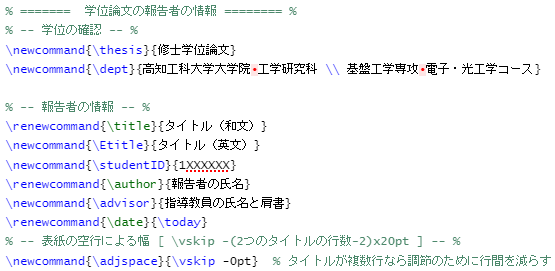
\includegraphics[keepaspectratio, width=0.9\linewidth]{verification_of_graduation.png}
  \caption{表紙の設定を記載する位置のスクリーンショット.main\_LuaTeX.texの$87$行目くらいにある.}
  \label{fig:cover}
\end{figure}
% === figure === %

\section{ヘッダー・フッターの設定}
今設定しているヘッダー・フッターは,ヘッダーに下線を入れて小口にページ番号,のどに章・節を記載している.
変える箇所は図\ref{fig:nomble}にある.設定したヘッダー・フッターの出力結果は図\ref{fig:header}にある.

% === figure === %
\begin{figure}[h]
  \centering
  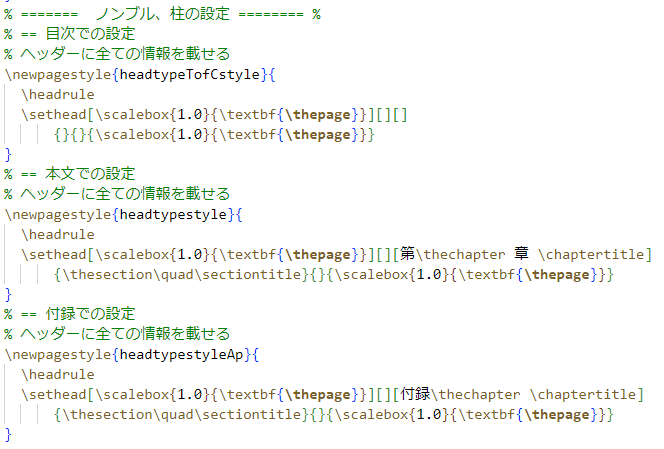
\includegraphics[keepaspectratio, width=0.9\linewidth]{nomble.png}
  \caption{ヘッダー・フッターの設定を記載した位置のスクリーンショット.main\_LuaTeX.texの$55$行目くらいにある.}
  \label{fig:nomble}
\end{figure}
% === figure === %
% === figure === %
\begin{figure}[h]
  \centering
  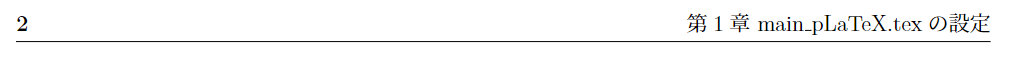
\includegraphics[keepaspectratio, width=0.9\linewidth]{header.png}
  \caption{ヘッダー・フッターの設定が反映された結果.}
  \label{fig:header}
\end{figure}
% === figure === %


\section{目次の設定について}
目次と図目次,表目次は,main\_LuaTeX.texの110--112行目で制御している.
図目次と表目次を入れるかは各指導教官の方々の指示に従うこと.
$2023$年度の「卒業研究報告書(学士論文)・修士論文の執筆要項」では
図目次と表目次についての記載はないため,不要かもしれない.
使用する場合は \% でコメントアウトを外せば良い.

\subsection{表目次について}
表\ref{tab:triangle}に適当な表を作成した.
表目次を確認すると表\ref{tab:triangle}がある.

% === table === %
\begin{table}[htbp]
  \centering
  \caption{三角関数と双曲線関数}
  \begin{tabular}{cc} \toprule 
    三角関数 & 双曲線関数 \\ \hline
    $\sin(x)$ & $\sinh(x)$ \\
    $\cos(x)$ & $\cosh(x)$ \\
    $\tan(x)$ & $\tanh(x)$ \\ \hline
  \end{tabular}
  \label{tab:triangle}
\end{table}
% === table === %


\subsection{図目次について}
図目次の動作は,図\ref{fig:cover}などを図目次と一致しているか確認すれば,
それぞれ対応する図ごとにページ番号が記載されていることがわかる.


\section{その他各種設定について}
上記の表紙やヘッダー・フッター,目次に加えて他にも,main\_LuaTeX.tex内の
\textbackslash graphicspath\{\{./figures/\}\}の設定などがあるが,
細かい設定なのでここでは割愛する.